\documentclass{beamer}

% Packages
\usepackage{tikz}
\usepackage{listings}
\usepackage{xcolor}
\usepackage{graphicx}

% Set image search paths
\graphicspath{{../images/}{../../shared/images/}}

% Custom colors
\definecolor{ds9blue}{RGB}{25,25,112}
\definecolor{ds9gold}{RGB}{218,165,32}
\definecolor{ds9grey}{RGB}{105,105,105}
\definecolor{ds9red}{RGB}{178,34,34}

% Theme setup
\usetheme{Madrid}
\usecolortheme[named=ds9blue]{structure}
\setbeamercolor{title}{fg=ds9gold,bg=ds9blue}
\setbeamercolor{frametitle}{fg=ds9blue,bg=ds9gold!20}

% Title page configuration
\title[Array Searching]{ Array Search Algorithms}
\subtitle{Linear and Binary Search Implementation}
\author[Mr. Gullo]{Mr. Gullo}
\date[Feb 2025]{February, 2025}

\begin{document}

\frame{\titlepage}

\begin{frame}{Learning Objectives}
\begin{itemize}
\item Understand the fundamental differences between linear and binary search
\item Analyze time complexity in simple terms
\item Read and comprehend C++ implementations of search algorithms
\item Identify appropriate use cases for each search method
\end{itemize}
\end{frame}

\begin{frame}{Linear Search: The Basics}
\begin{columns}
\column{0.5\textwidth}
\begin{itemize}
\item Searches through array elements one by one
\item Works on both sorted and unsorted arrays
\item Time complexity: O(n)
\end{itemize}

\column{0.6\textwidth}
\begin{figure}
    \centering
    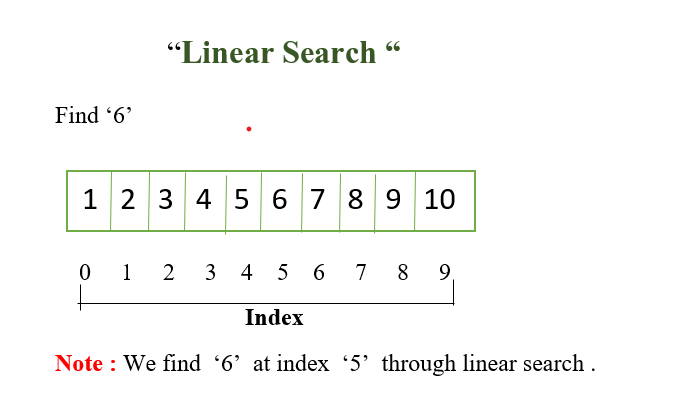
\includegraphics[width=1\linewidth]{cs12-searching-linear-search-example.png}
\end{figure}
\end{columns}
\end{frame}

\begin{frame}[fragile]{Linear Search Implementation}
\begin{lstlisting}[language=C++]
bool search_unsorted(int value, int arr[], int length){
   for(int i = 0; i < length; i++)
      if(value == arr[i]) return true;
   return false;
}
\end{lstlisting}
\pause

\begin{itemize}
\item Simple implementation
\item Checks each element exactly once
\item Returns as soon as value is found
\end{itemize}
\end{frame}

\begin{frame}{Binary Search: The Concept}
\begin{columns}
\column{0.3\textwidth}
\begin{itemize}
\item Requires sorted array
\item Divides search space in half
\item Time complexity: O(log n)
\end{itemize}

\column{0.6\textwidth}
\begin{figure}
    \centering
    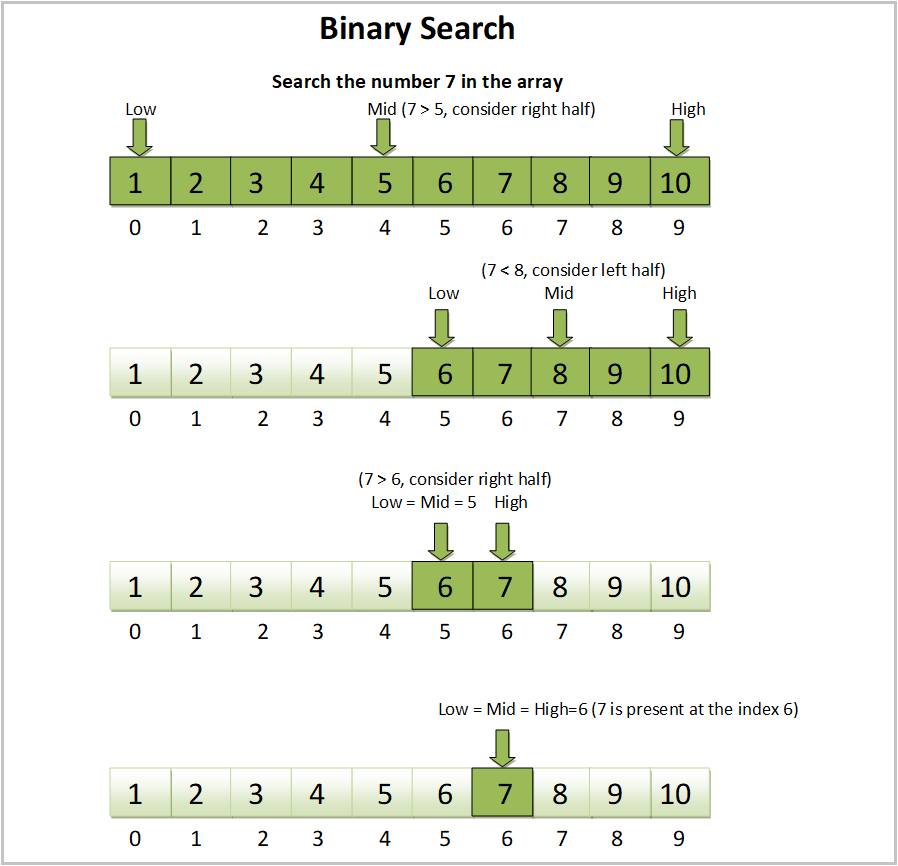
\includegraphics[width=1\linewidth]{../images/cs12-arrays-search_visualization.png}
\end{figure}
\end{columns}
\end{frame}

\begin{frame}[fragile]{Binary Search Implementation}
\begin{lstlisting}[language=C++]
bool search_sorted(int value, int arr[], int length) {
    // Initialize indices for binary search
    int firstIndex = 0;
    int lastIndex = length - 1;    
    while(firstIndex <= lastIndex) {
        // TODO 1: Calculate the middle index
        int midpointIndex =   "..."      
        // TODO 2: Check if value found
        if(check if current element is target) 
        { "..." return true;   }
        // TODO 3: Decide which half to search
        else if(check if search right half) {
        "... "}
        else {// update the index to search left half
        }    } return false;    }
\end{lstlisting}
\end{frame}

 \begin{frame}{Project Structure Overview}
\begin{columns}
\column{0.6\textwidth}
\begin{itemize}
\item Multi-file organization:
  \begin{itemize}
  \item Header file (\texttt{arraySearch.h})
   \item Main program (\texttt{main.cpp})
   \item Implementation (\texttt{arraySearch.cpp})
  \end{itemize}
  \pause

\item Separation of debugging concerns
\pause
\item Improved maintainability
\end{itemize}
\pause

\column{0.4\textwidth}
\begin{block}{\texttt{arraySearch.h}}
Header Definitions
\end{block}
\vspace{-0.3cm}
\begin{align*}
\uparrow \hspace{2cm} \uparrow
\end{align*}
\vspace{-0.8cm}
\begin{columns}
\column{0.5\textwidth}
\begin{block}{\texttt{.cpp}}
Implementation
\end{block}
\column{0.5\textwidth}
\begin{block}{\texttt{main}}
Program
\end{block}
\end{columns}
\end{columns}
\end{frame}

\begin{frame}[fragile]{Header File: arraySearch.h}
\begin{lstlisting}[language=C++, basicstyle=\small]
#ifndef ARRAYSEARCH_H_INCLUDED
#define ARRAYSEARCH_H_INCLUDED

bool search_unsorted(int value, int arr[], int length);
   // Returns true if value is in the array. else False.
   // Note: this should be O(n)

bool search_sorted(int value, int arr[], int length);
   // Returns true if value is in the array. eslse False.
   // Note: this should be O(log(n))

bool test_search_unsorted(); //static edge case testing
bool test_search_sorted(); //static edge case testing
#endif
\end{lstlisting}
\pause

\begin{itemize}
\item Function declarations only
\item Include guards prevent multiple inclusion
\item Clear documentation of function behavior
\end{itemize}
\end{frame}

\begin{frame}[fragile]{Main Program Structure}
\begin{lstlisting}[language=C++, basicstyle=\small]
int main() {
    // Create test array
    int testArray[] = {2, 5, 8, 12, 16, 23, 38, 56, 72, 91};
    int length = sizeof(testArray)/sizeof(testArray[0]);
    
    // Test values
    int searchValues[] = {16, 91, 2, 50, -5, 100};
    
    // Test both search functions
    cout << "\n=== Testing Linear Search ===\n";
    // ... testing code ...
    
    cout << "\n=== Testing Binary Search ===\n";
    // ... testing code ...
    
    return 0;}
\end{lstlisting}


\begin{itemize}
\item Organized testing structure
\item Clear separation of test data and logic
\end{itemize}
\end{frame}

\begin{frame}{Testing Implementation}
\begin{itemize}
\item Comprehensive test cases:
  \begin{itemize}
  \item Elements at beginning, middle, and end
  \item Values not in array
  \item Edge cases (empty array, single element)
  \end{itemize}
\item Automated testing functions:
  \begin{itemize}
  \item \texttt{test\_search\_unsorted()}
  \item \texttt{test\_search\_sorted()}
  \end{itemize}
\end{itemize}

\begin{columns}[t]
\column{0.32\textwidth}
\begin{block}{Present Values}
Expected: Success
\end{block}

\column{0.32\textwidth}
\begin{block}{Missing Values}
Expected: Failure
\end{block}

\column{0.32\textwidth}
\begin{block}{Edge Cases}
Expected: Validation
\end{block}
\end{columns}
\end{frame}


\begin{frame}{Comparison: When to Use Each}
\begin{columns}
\column{0.5\textwidth}
\textbf{Linear Search}
\begin{itemize}
\item Unsorted data
\item Small arrays
\item One-time searches
\end{itemize}

\pause

\column{0.5\textwidth}
\textbf{Binary Search}
\begin{itemize}
\item Sorted data
\item Large datasets
\item Frequent searches
\end{itemize}
\end{columns}
\end{frame}

\begin{frame}{Summary}
\begin{itemize}
\item Linear search is simple but slower (O(n))
\item Binary search requires sorted data but is faster (O(log n))
\item Choice depends on:
  \begin{itemize}
  \item Data organization
  \item Dataset size
  \item Search frequency
  \end{itemize}
\item Testing is crucial for both implementations
\end{itemize}
\end{frame}

\end{document}